% Lecture 21

\section{The Counit Weak Equivalence}

\lecture[]{2022-01-10}

\subsection{The Singular Complex Functor is Homotopical}

Our next step\rightnote{\Attention\ I missed this lecture, one should definitely refer to \href{https://www.math.uni-bonn.de/people/schwede/sset_vs_spaces.pdf}{Prof. Schwede's own notes}} in showing the \enquote{correspondence} of spaces and simplicial sets is to show that for every space $Z$, the adjunction counit $\epsilon_Z:|\S(Z)|\to Z$ is a weak equivalence. Today we begin by showing that $\S:\Top\to\sSet$ takes weak equivalences to homotopy equivalences and we start to study the homology of the geometric realization.

Recall the adjunction
\[
\sSet\underset{\S}{\overset{|-|}{\leftrightarrows}}\Top,
\]
the data of which is a bijection
\[\Hom_\Top(|X|,A)\cong\Hom_\sSet(X,\S(A))\]
natural in the simplicial set $X$ and the topological space $A$.

Equivalently, we may specify the components of the adjunction unit $\eta_X:X\to\S|X|$, i.e. \[(\eta_X)_n:X_n\to(\S|X|)_n=\Hom_\Top(\ns,|X|),\quad x\mapsto(t\mapsto[x,t]),\]
and the adjunction counit, i.e. the continuous map \[\epsilon_Z:|\S(Z)|\to Z,\quad [f,t]\mapsto f(t).\]

We want the adjunction bijection to pass to an analogous bijection of homotopy classes.

\begin{proposition}\label{proposition:adjunction-preserves-homotopy}
Let $A$ be a space and $X$ a simplicial set. Then two continuous maps $f,g:|X|\to A$ are homotopic if and only if their adjoint $f^\flat,g^\flat:X\to\S(A)$ are simplicially homotopic.
\end{proposition}

\begin{proof}
$(\implies)$ Let $H:|X|\times\sx{1}\to A$ be a homotopy from $f$ to $g$, in the sense that $H(-,(0,1))=f$ and $H(-,(1,0))=g$. We define a morphism of simplicial sets $K:X\times\Delta^1\to\S(|X|\times\sx{1})$ by:
\begin{align*}
    K_n:X_n\times\Delta([n],[1])&\to\Hom_\Top(\ns,|X|\times\sx{1})\\
    (x,\alpha)&\mapsto K_n(x,\alpha)(t)=([x,t],\alpha_*(t))
\end{align*}
The desired simplicial homotopy from $f^\flat$ to $g^\flat$ is then the composite
\[X\times\Delta^1\xto{K}\S(|X|\times\sx{1})\xto{\S(H)}\S(A).\]
$(\impliedby)$ Suppose that $f^\flat$ and $g^\flat$ are simplicially homotopic. Since being homotopic for space maps is an equivalence relation (in particular symmetric and transitive), we can assume without loss of generality that $f^\flat$ and $g^\flat$ are related by an elementary homotopy
\[K:X\times\Delta^1\to\S(A)\]
from $f^\flat$ to $g^\flat$.

The desired homotopy between $f$ and $g$ is then the composite
\[|X|\times\sx{1}\xto{\cong}|X\times\Delta^1|\xto{|K|}|\S(A)|\xto{\epsilon_A}A\]
where the first map is the inverse of the map
\[|X\times\Delta^1|\xto{(|p_1|,|p_2|)}|X|\times|\Delta^1|\cong|X|\times\sx{1}\]
which was proved to be an homeomorphism in AT1Sheet11.2.
\end{proof}

\begin{theorem}\label{theore:singular-complex-functor-is-homotopical}
Let $f:A\to B$ be a weak homotopy equivalence of spaces. Then $\S(f):\S(A)\to\S(B)$ is a homotopy equivalence of simplicial sets.
\end{theorem}

\begin{proof}
Since $f$ is a weak equivalence, for every CW-complex $K$ the induced map
\[f_*:=[K,f]:[K,A]\to[K,B]\]
is bijective, as shown in ATSheet10.2. For $K=|\S(B)|$, we get a bijection
\[
f_*:[|\S(B)|,A]\xto{\cong}[|\S(B)|,B],
\]
So there is a continuous map $\lambda:|\S(B)|\to A$, unique up to homotopy, such that $f\circ\lambda\simeq\epsilon_B$.

The adjoint $\lambda^\#:\S(B)\to\S(A)$ is a morphism of simplicial sets and by proposition \ref{proposition:adjunction-preserves-homotopy} we have that $\S(f)\circ\lambda^\#$ is simplicially homotopic to $(\epsilon_B)^\#=\id_{\S(B)}$. To see that the other composite $\lambda^\#\circ\S(f):\S(A)\to\S(A)$ is simplicially homotopic to $\id_{\S(A)}$ we observe that
\[f\circ\lambda\circ|\S(f)|\simeq\epsilon_B\circ|\S(f)|=f\circ\epsilon_A\]
where the last equality is by naturality of $\epsilon$. Since there is a bijection
\[f_*[|\S(A)|,A]\xto{\cong}[|\S(A)|,B]\]
we can conclude that $\lambda\circ|\S(f)|$ is homotopic to $\epsilon_A$. Again, thanks to proposition \ref{proposition:adjunction-preserves-homotopy} passing to the adjoints lets us conclude.
\end{proof}

\subsection{Homology of the Geometric Realization}

We now want to prove that for any simplicial set $X$ and any coefficient group $A$, the adjunction unit $\eta_X:X\to\S|X|$ induces an isomorphism
\[H_n(\eta_X):H_n(X;A)\to H_n(|X|;A)\]
from the homology of the simplicial set to the singular homology of the geometric realization. As a corollary we will deduce that for every space $Z$, the adjunction counit $\epsilon_Z:|\S(Z)|\to Z$ induces isomorphisms of all singular homology groups.

\begin{theorem}\label{theorem:simplicial-and-singular-homology}
For any simplicial set $X$, the map
\[H_*(\eta_X):H^\simpl_*(X;\Z)\to H^\simpl_*(\S|X|;\Z)=H^\sing_*(|X|;\Z)\]
is an isomorphism.
\end{theorem}

We will prove a relative version of the theorem for pairs of simplicial sets $(K,L)$, i.e. with $L\subset K$ a simplicial subset.

Observe first that the adjunction units and the inclusions induce a commutative square of chain complexes:
\[
\begin{tikzcd}
C_*(L;A) \ar[d,"C_*(\eta_L;A)"] \ar[r,hook] & C_*(K;A) \ar[d,"C_*(\eta_K;A)"]\\
C_*(\S|L|;A) \ar[r,hook] & C_*(\S|K|;A)
\end{tikzcd}
\]
We write
\[\eta_{K,
L}:C_*(K;A)/C_*(L;A)\to C_*(\S|K|;A)/C_*(\S|L|;A)\]
for the chain map induced on quotient complexes. Recall that the homology of the chain complex $C_*(K;A)/C_*(L;A)$ is the relative homology $H_*(K,L;A)$ of the pair of simplicial sets $(K,L)$; similarly, the homology of $C_*(\S|K|;A)/C_*(\S|L|;A)$ is the relative homology $H_*(|K|,|L|;A)$ of the space pair $(|K|,|L|)$.

Now we are ready to prove the relative version of theorem \ref{theorem:simplicial-and-singular-homology}.

\begin{theorem}\label{theorem:simplicial-and-singular-relative-homology}
For every pair $(K,L)$ of simplicial sets and any abelian group $A$, the chain map $\eta_{K,L}$ is a quasi-isomorphism. In particular, the induced morphism
\[H_n(\eta_{K,L}):H_n(K,L;A)\to H_n(|K|,|L|;A)\]
is an isomorphism for all $n\ge0$.
\end{theorem}

\begin{proof}\renewcommand{\qedsymbol}{\textit{To be continued...}}
We subdivide the proof in $6$ claims.

Claim 1. Let $(M,N)$ and $(K,L)$ be two pairs of simplicial sets that participate in a pushout square of simplicial sets:
\[
\begin{tikzcd}
N \ar[r,hook] \ar[d,"f|_N"'] & M \ar[d,"f"]\\
L \ar[r,hook] & K
\end{tikzcd}
\]
If the theorem holds for $(M,N)$ it holds also for $(K,L)$.

\begin{claimproof}
The pushout square induces a commutative square of chain complexes:
\[
\begin{tikzcd}[row sep=large,column sep=large]
C_*(M;A)/C_*(N;A) \ar[r,"\eta_{M,N}","\simeq"'] \ar[d,"C_*(f)"'] & C_*(\S|M|;A)/C_*(\S|N|;A)) \ar[d,"C_*(\S|f|)"]\\
C_*(K;A)/C_*(L;A) \ar[r,"\eta_{K,L}"] & C_*(\S|K|;A)/C_*(\S|L|;A)
\end{tikzcd}\tag{$*$}
\]
The left vertical map in $(*)$ is an isomorphism of chain complexes because the map $f:M\to K$ restricts to bijections $M_n/N_n\to K_n/L_n$ for every $n\ge0$ (the original square being a pushout).
Moreover, $|f|$ induces on homology groups the map
\[|f|_*:H_n(|M|,|N|;A)\to H_n(|K|,|L|;A)\]
and since the square
\[
\begin{tikzcd}
{|N|} \ar[r,hook] \ar[d,"{|f|}|_{|N|}"'] & {|M|} \ar[d,"{|f|}"]\\
{|L|} \ar[r,hook] & {|K|}
\end{tikzcd}
\]
is a pushout of spaces (because realization is a left adjoint) and the horizontal maps are inclusions of CW-complexes, excision implies that the map of relative homology groups is an isomorphism (alternatively, one can notice that the additional cells of $|M|$ map bijectively, hence there is an isomorphism on relative cellular homology groups and therefore on singular homology groups). The upper horizontal map in $(*)$ is a quasi-isomorphism by hypothesis, hence the lower horizontal map is also a quasi-isomorphism.
\end{claimproof}

Claim 2. Let $(K,L,M)$ be a triple of simplicial sets. If the theorem holds for two of the three pairs $(K,L)$, $(K,M)$ and $(L,M)$, then it also holds for the third pair.

\begin{claimproof}
We obtain two triples of chain complexes
\[
\begin{tikzcd}
C_*(M;A) \ar[r,hook] \ar[d,"C_*(\eta_M)"] & C_*(L;A) \ar[r,hook] \ar[d,"C_*(\eta_L)"] & C_*(K;A) \ar[d,"C_*(\eta_K)"]\\
C_*(\S|M|;A) \ar[r,hook] & C_*(\S|L|;A) \ar[r,hook] & C_*(\S|K|;A)
\end{tikzcd}
\]
and from these we form two short exact sequences of chain complexes, which combine in a diagram:
{\small\[
\begin{tikzcd}[column sep=2.5ex]
0 \ar[r] & C_*(L;A)/C_*(M;A) \ar[r] \ar[d,"C_*(\eta_{L,M})"] & C_*(K;A)/C_*(M;A) \ar[r] \ar[d,"C_*(\eta_{K,M})"] & C_*(K;A)/C_*(L;A) \ar[d,"C_*(\eta_{K,L})"] \ar[r] & 0\\
0 \ar[r] & C_*(\S|L|;A)/C_*(\S|M|;A) \ar[r] & C_*(\S|K|;A)/C_*(\S|M|;A) \ar[r] & C_*(\S|K|;A)/C_*(\S|L|;A) \ar[r] & 0
\end{tikzcd}
\]}

We apply the $5$-lemma to the resulting commutative diagram of long exact homology sequences: since the theorem holds for two of the three pairs, every two out of three vertical morphisms of
homology groups are isomorphism, hence so are the remaining ones. Therefore the theorem holds for the
third pair, which proves the claim.
\end{claimproof}

Claim 3 The theorem holds for the pair $(\Delta^m,\de\Delta^m)$ for all $m\ge0$.

\begin{claimproof}
We argue by induction on $m$. For $m=0$, $\Delta^0$ is a constant simplicial set with one vertex and $\de\Delta^m=\emptyset$; consequently, the space $|\Delta^0|$ consists of a single point, while $|\de\Delta^0|$ is empty. Hence in this case both $H_*(\Delta^0,\de\Delta^0;A)$ and $H_*(|\Delta^0|,|\de\Delta^0|;A)$ consist of a copy of $A$ concentrated in dimension $0$ and the map $\eta_{\Delta^0,\de\Delta^0}$ is a quasi-isomorphism.

For $m\ge1$, we let $\Lambda^m_0$ denote the \enquote{$0$-th horn} of $\Delta^m$, i.e. the simplicial subset generated by $d_1,\dots,d_m:[m-1]\to[m]$.
\[
\Lambda^1_0 = 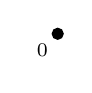
\begin{tikzpicture}[baseline=-.15em]
\filldraw (0,0) circle (2pt) node[anchor=north east]{\scriptsize0};
\end{tikzpicture}
\quad\quad\quad
\Lambda^2_0 = 
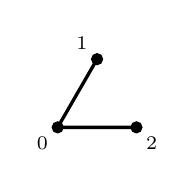
\begin{tikzpicture}[baseline=0.5em]
\draw[very thick]
(1,0)--(0,0)--(.5,.866);
\filldraw
(1,0) circle (2pt) node[anchor=north west]{\scriptsize2}
(0,0) circle (2pt) node[anchor=north east]{\scriptsize0}
(.5,.866) circle (2pt) node[anchor=south east]{\scriptsize1};
\end{tikzpicture}
\quad\quad\quad
\Lambda^3_0 =
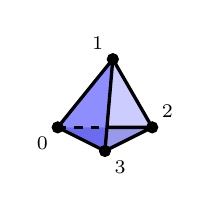
\begin{tikzpicture}[baseline=0.5em]
\fill[blue!20] (-.2,0)--(1,0)--(.5,.866);
\fill[blue!80!black, opacity=0.4] (-.2,0)--(.4,-.3)--(1,0);
\fill[blue, opacity=0.3] (-.2,0)--(.4,-.3)--(.5,.866);
\draw[very thick]
(.4,-.3)--(-.2,0)--(.5,.866)
(.5,.866)--(.4,-.3)--(1,0)--(.5,.866)
(1,0)--(.45,0);
\draw[very thick, dashed]
(-.2,0)--(.45,0);
\filldraw
(1,0) circle (2pt) node[anchor=south west]{\scriptsize2}
(-.2,0) circle (2pt) node[anchor=north east]{\scriptsize0}
(.5,.866) circle (2pt) node[anchor=south east]{\scriptsize1}
(.4,-.3) circle (2pt) node[anchor=north west]{\scriptsize3};
\end{tikzpicture}
\]

Then both $\Delta^m$ and $\Lambda^m_0$ are simplicially contractible, and their geometric realizations $|\Delta^m|$ and $|\Lambda^m_0|$ are contractible. So the relative homology groups $H_*(\Delta^m,\Lambda^m_0;A)$ and $H_*(|\Delta^m|,|\Lambda^m_0|;A)$ are all trivial and $\eta_{\Delta^0,\Lambda^m_0}$ is a quasi-isomorphism. The simplex $d_0:[m-1]\to[m]$ is the unique non degenerate simplex of $\de\Delta^m$ that does not belong to $\Lambda^m_0$. Hence the following square is a pushout of simplicial sets:
\[
\begin{tikzcd}
\de\Delta^{m-1} \ar[d,"(d_0)_*"'] \ar[r,"\incl"] & \Delta^{m-1} \ar[d,"(d_0)_*"]\\
\Lambda^m_0 \ar[r,"\incl"] & \de\Delta^m
\end{tikzcd}
\]
Since the theorem holds for the pair $(\Delta^{m-1},\de\Delta^{m-1})$ by induction, it holds for the pair $(\de\Delta^m,\Lambda^m_0)$ by Claim 1. Since the theorem holds for the pairs $(\Delta^m,\Lambda^m_0)$ and $(\de\Delta^m,\Lambda^m_0)$, it holds for the pair $(\Delta^m,\de\Delta^m)$ by Claim 2, which concludes the inductive step.
\end{claimproof}

Claim 4. Suppose that the theorem holds for a family $\cb{(K_i,L_i)}_{i\in I}$ of pairs of simplicial sets. Then the theorem also holds for the pair $(\amalg_{i\in I}K_i,\amalg_{i\in I}L_i)$ of disjoint unions.

\begin{claimproof}
The geometric realization and singular complex functors both preserve disjoint unions, and the functor $C_*(-;A)$ takes disjoint unions of simplicial sets to direct sums of chain complexes. So in the commutative square
\[
\begin{tikzcd}[column sep=large]
\bigoplus_{i\in I} C_*(K_i;A)/C_*(L_i;A) \ar[d,"\cong"'] \ar[r,"\bigoplus\eta_{K_i,L_i}"] & \bigoplus_{i\in I} C_*(\S|K_i|;A)/C_*(\S|L_i|;A) \ar[d,"\cong"]\\
C_*(\amalg\,K_i;A)/C_*(\amalg\, L_i;A) \ar[r,"\eta_{\amalg K_i,\amalg L_i}"] & C_*(\S|\amalg K_i|;A)/C_*(\S|\amalg L_i|;A)
\end{tikzcd}
\]
the canonical vertical maps are isomorphisms. Any direct sum of quasi-isomorphism is a quasi-isomorphism, so the upper horizontal morphism is a quasi-isomorphism since all pairs $(K_i,L_i)$ satisfy the hypothesis of the theorem. Hence the lower horizontal maps is a quasi-isomorphism by Claim 1, as we wanted to show.
\end{claimproof}

\end{proof}
